\chapter{BaseLib Level 4}
\chaptermark{Level 4}

BaseLib Level 4 integrate full HTTP protocol, server and client side. The server can manage more than one client at a time and the stream is usually coded in HTML version 1.0 with support to the \textit{keep alive} functionality. There is also an approach to manage secure connection letting the developer which pages are for public domain and which are only for selected users defining a sort of policy security.



\section{HttpStream and URLs}


\begin{figure}[h!]
 \begin{center}
  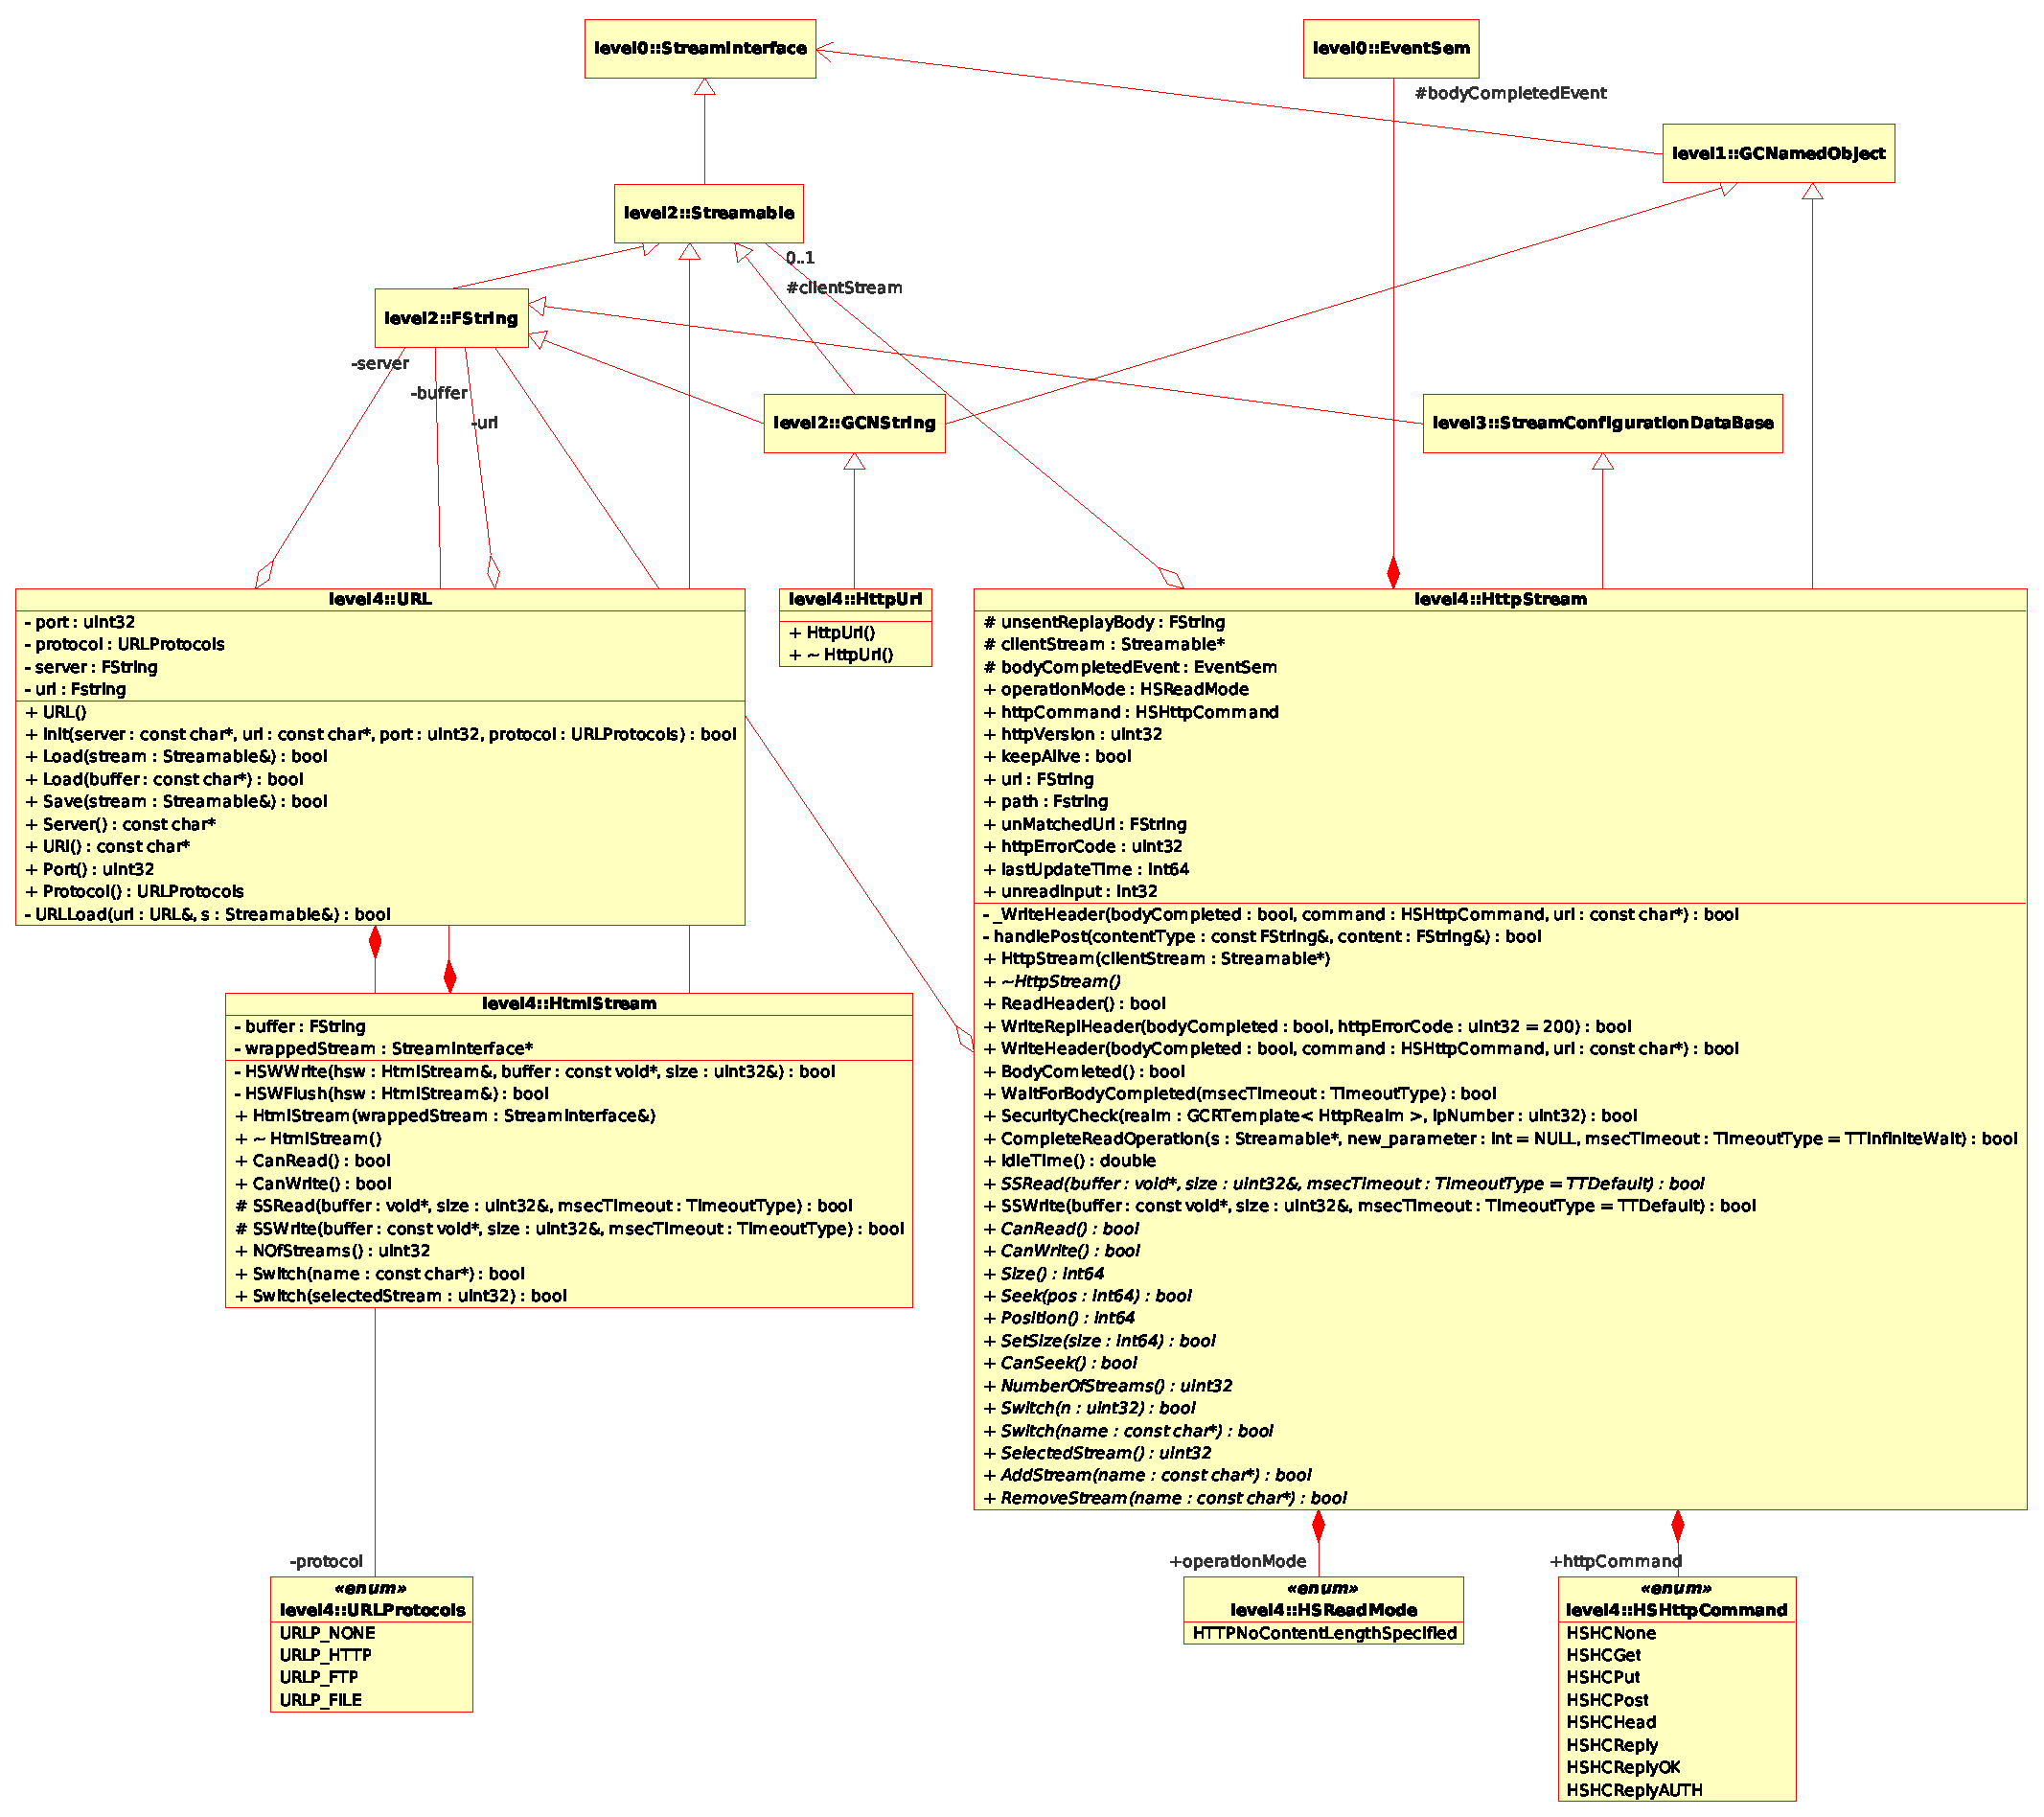
\includegraphics[width=\textwidth]{level4/level4-HttpStream.eps}
  \caption{BaseLib Level 4 HttpStream and URLs infrastructure}
  \label{f:level4:HttpStream}
 \end{center}
\end{figure}

Figure \ref{f:level4:HttpStream} depicts an UML schema of the classes involved in this section. Classes in this section are:
\begin{itemize}
 \item URL
 \item HttpURL

 \item HttpStream
 \item HtmlStream
\end{itemize}



\subsubsection{HttpStream}
\texttt{[HttpStream.h, HttpStream.cpp]}\\
The class \texttt{HttpStream} implements an HTTP language multiple stream. The main stream \textit{read} and \textit{write} channels, operate with the client (or on a cache until method \texttt{CompleteReadOperation} is not called); the other streams allow read/write access to special information like \texttt{HttpOptions} or HTML form commands.
The HTTP options are accessed using the streams whose name begins with \texttt{InputHttpOtions} or \texttt{OutputHttpOptions}. \texttt{InputCommands} contain the informations produced by submitting a form. The stream called \texttt{Peer} contains the name of the connecting peer.\\


The class \texttt{HttpStream} inherits from \texttt{GCNamedObject} and \texttt{StreamConfigurationDataBase}.
The first attribute, \texttt{unsentReplyBody}, is the part of the reply that is not sent yet; the second, \texttt{clientStream} is the stream connected to the remote client that should implement a timeout for read operation and translation for specific HTTP hex char groups; \texttt{bosyCompletedEvent} is a semaphore on which to wait for body completed.\\


Then come the public attributes. The attribute \texttt{operationMode} represents one of the following the values: \texttt{writeToString}, \texttt{writeToClient}, \texttt{writeToCDB}. The attribute \texttt{httpCommand} stores what command was requested; this affects the working of \texttt{Read} and \texttt{Write} methods, i.e. \texttt{Write} method on the main channel does not work for HTTP HEAD tag; it can also be the reply, in which case it contains the reply code. \texttt{httpVersion} holds the HTTP version number, i.e. \texttt{1000} means \textit{v1.0}, \texttt{2100} means \textit{v2.1}.
The attribute \texttt{keepAlive} is \texttt{true} if the communication should continue after transaction; the \texttt{url} is the URL of the requested page, the same information is also holded by the \texttt{path} attribute that store it with ``.'' (dotted notation) instead of ``\/''. \texttt{unMatchedUrl} stores the remainder of url not matched in the search. \texttt{httpErrorCode} sves the HTTP return code; the attribute \texttt{lastUpdateTime} is the last time the body has been updated and \texttt{unreadInput} is how much data is still waiting in the input stream from the client.
\begin{lstlisting}[
extendedchars=true,%
basicstyle=\fontfamily{pcr}\fontseries{m}\selectfont\footnotesize, %
stepnumber=1,%
numberstyle=\tiny,%
keywordstyle=\footnotesize\tt ,%
language=C++]
protected:
   FString unsentReplyBody;
   Streamable* clientStream;
   EventSem bodyCompletedEvent;
public:
   HSOperatingMode operationMode;
   HSHttpCommand httpCommand;
   uint32 httpVersion;
   bool keepAlive;
   FString url;
   FString path;
   FString unMatchedUrl;
   uint32 httpErrorCode;
   int64 lastUpdateTime;
   int32 unreadInput;
\end{lstlisting}


The method \texttt{handlePost} handles a post request. The constructor builds an empty class, and the destructor simply destroies it.


The method \texttt{ReadHeader} reads the HTTP header and leaves body up to the user; \texttt{WriteReplyHeader} begins an HTTP reply message: sends out the HTTP header as currently formed and the outstanding body; any further write will operate directly on the stream; if \texttt{complete} is \texttt{true} then the whole body has been cached and therefore we can announce the body size. \texttt{WriteHeader} begins an HTTP message: sends out the HTTP header as currently formed and the outstanding body; any further write will operate directly on the stream if complete is \texttt{true} then the whole body has been cached and therefore we can announce the body size, if \texttt{command} is a reply we are generating a reply message.\\


The method \texttt{BodyCompleted} returns \texttt{true} if the writing of the body has been completed. \texttt{WaitForbodyCompleted} is a sender thread that waits for the completion of this activity.


The method \texttt{SecurityCheck} checks a request against a security module; \texttt{CompleteReadOperation} completes the reading of an HTTP message throwing away the content. \texttt{IdeleTime} returns how long since the last write operation.
\begin{lstlisting}[
extendedchars=true,%
basicstyle=\fontfamily{pcr}\fontseries{m}\selectfont\footnotesize, %
stepnumber=1,%
numberstyle=\tiny,%
keywordstyle=\footnotesize\tt ,%
language=C++]
   bool _WriteHeader(bool bodyCompleted,HSHttpCommand command,const char* url);
private:
   bool handlePost(const FString& contentType, FString& content);
public:
   HttpStream(Streamable *clientStream);
   virtual ~HttpStream();

   bool ReadHeader();
   bool WriteReplyHeader(bool bodyCompleted,uint32 httpErrorCode=200);
   inline bool WriteHeader(bool bodyCompleted,HSHttpCommand command,const char* url);

   bool BodyCompleted();
   bool WaitForBodyCompleted(TimeoutType msecTimeout);

   bool SecurityCheck(GCRTemplate<HttpRealm> realm,uint32 ipNumber);
   bool CompleteReadOperation(Streamable* s=NULL,TimeoutType msecTimeout=TTInfiniteWait);
   double IdleTime();
\end{lstlisting}

Other methods, that follow, override the \texttt{Streamable} ones, we report them for a documnentation purpose.

\begin{lstlisting}[
extendedchars=true,%
basicstyle=\fontfamily{pcr}\fontseries{m}\selectfont\footnotesize, %
stepnumber=1,%
numberstyle=\tiny,%
keywordstyle=\footnotesize\tt ,%
language=C++]
   virtual bool SSRead(void* buffer,uint32& size,TimeoutType msecTimeout=TTDefault);
   virtual bool SSWrite(const void* buffer,uint32& size,TimeoutType msecTimeout=TTDefault);
   virtual bool CanRead();
   virtual bool CanWrite();

   virtual int64 Size();
   virtual bool Seek(int64 pos);
   virtual bool CanSeek();
   virtual int64 Position();
   virtual bool SetSize(int64 size);

   virtual uint32 NumberOfStreams();
   virtual bool Switch(uint32 n);
   virtual bool Switch(const char* name);
   virtual uint32 SelectedStream();
   virtual bool AddStream(const char* name);
   virtual bool RemoveStream(const char* name);
\end{lstlisting}



\section{HttpInterface and HttpRealm}


\begin{figure}[h!]
 \begin{center}
  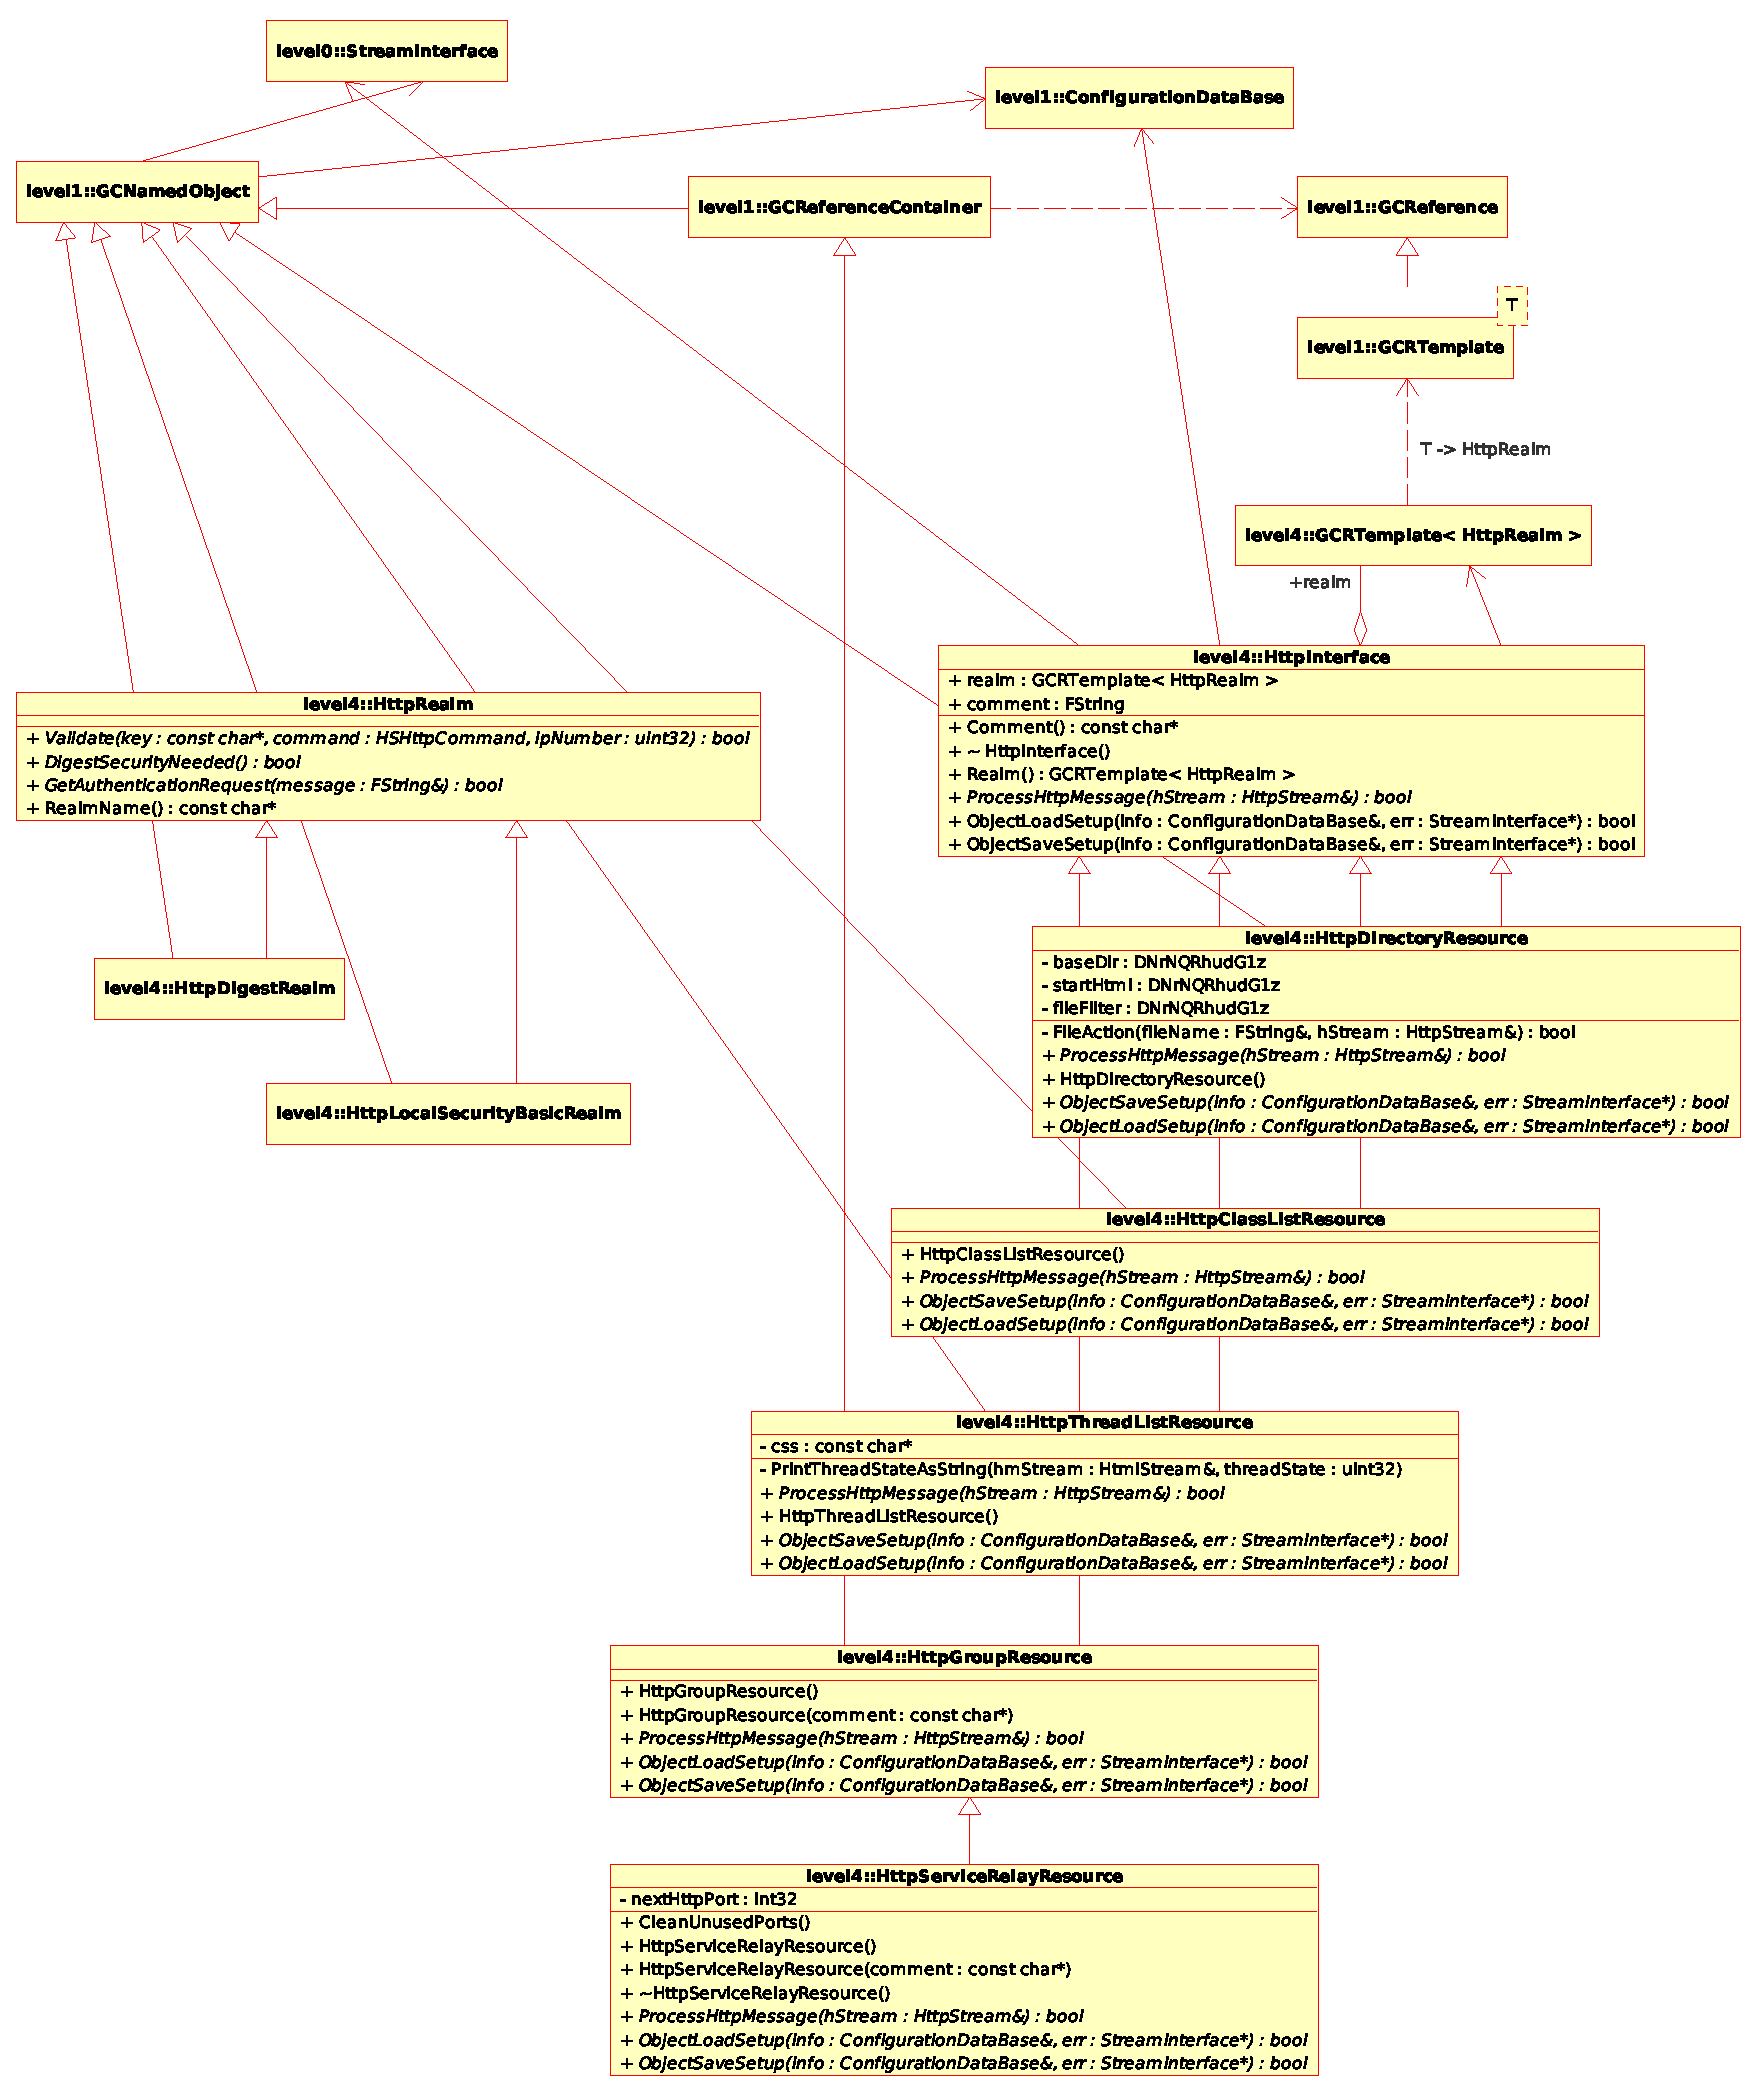
\includegraphics[width=0.88\textwidth]{level4/level4-HttpInterface.eps}
  \caption{BaseLib Level 4 HttpInterface and HttpRealm}
  \label{f:level4:HttpInterface}
 \end{center}
\end{figure}

Figure \ref{f:level4:HttpInterface} depict an UML diagram of classes in this section. Classes in this section are (the first three are from the security suite and the others comes from the \texttt{HttpInterface} hierarchy):
\begin{itemize}
 \item HttpRealm
 \item HttpDigestRealm
 \item HttpLocalSecurityBasicRealm

 \item HttpInterface
 \item HttpDirectoryResource
 \item HttpClassListResource
 \item HttpThreadListResoource
 \item HttpGroupResource
 \item HttpService RelayResource
\end{itemize}



\subsubsection{HttpInterface}
\texttt{[HttpInterface.h]}\\
The class \texttt{HttpInterface} is the base class for a generic HTTP resource object; each resource object that wants to share its state or part of its state via the BaseLib HTTP server must inherits this interface and overriddes the \texttt{ProcessHttpMessage} method.

In the overridden \texttt{ProcessHttpMessage} the subclass must output an HTTP page about the state of the class.\\


The method \texttt{GCRTemplate<HttpRealm>} is a reference to the \textit{realm} database, i.e. a container of security options; \texttt{comment} is the page name to be presented to the viewer.


The method \texttt{Comment} return \texttt{comment.Buffer()}; \texttt{Realm} method return a reference to the \texttt{realm} database. The method \texttt{ProcessHttpMessage} is the method that will be overridden to obtain an HTTP page for the subclassed object.

The method \texttt{ObjectLoadSetup} calls \texttt{realm}'s one that is inherited from the \texttt{GCRTemplate}; the method \texttt{ObjectSaveSetup} behave the same as \texttt{ObjectLoadSetup}.

\begin{lstlisting}[
extendedchars=true,%
basicstyle=\fontfamily{pcr}\fontseries{m}\selectfont\footnotesize, %
stepnumber=1,%
numberstyle=\tiny,%
keywordstyle=\footnotesize\tt ,%
language=C++]
public:
   GCRTemplate<HttpRealm> realm;
   FString comment;

public:
   virtual ~HttpInterface(){};
   const char* Comment();
   GCRTemplate<HttpRealm> Realm();
   virtual bool ProcessHttpMessage(HttpStream& hStream)=0;
   bool ObjectLoadSetup(ConfigurationDataBase& info,StreamInterface* err);
   bool ObjectSaveSetup(ConfigurationDataBase& info,StreamInterface* err);
\end{lstlisting}


